% Тут используется класс, установленный на сервере Papeeria. На случай, если
% текст понадобится редактировать где-то в другом месте, рядом лежит файл matmex-diploma-custom.cls
% который в момент своего создания был идентичен классу, установленному на сервере.
% Для того, чтобы им воспользоваться, замените matmex-diploma на matmex-diploma-custom
% Если вы работаете исключительно в Papeeria то мы настоятельно рекомендуем пользоваться
% классом matmex-diploma, поскольку он будет автоматически обновляться по мере внесения корректив
%
\documentclass{matmex-diploma}
\begin{document}
% Год, город, название университета и факультета предопределены,
% но можно и поменять.
% Если англоязычная титульная страница не нужна, то ее можно просто удалить.
\filltitle{ru}{
    chair              = {Кафедра системного программирования},
    title              = {Визуализация кода встроенных языков \\в Microsoft
Visual Studio},
    % Здесь указывается тип работы. Возможные значения:
    %   coursework - Курсовая работа
    %   diploma - Диплом специалиста
    %   master - Диплом магистра
    %   bachelor - Диплом бакалавра
    type               = {coursework},
    position           = {студента},
    group              = 242,
    author             = {Озерцов Александр Сергеевич},
    supervisorPosition = {ст.пр., магистр},
    supervisor         = {Григорьев С.\,В.},
    reviewerPosition   = {ст. преп.},
    reviewer           = {Вербицкая Е.\,А.},
    chairHeadPosition  = {д.\,ф.-м.\,н., профессор},
    chairHead          = {Хунта К.\,Х.},
%   university         = {Санкт-Петербургский Государственный Университет},
%   faculty            = {Математико-механический факультет},
%   city               = {Санкт-Петербург},
%   year               = {2013}
}

\maketitle
\tableofcontents
% У введения нет номера главы

\section*{Введение}
\subsection*{Встроенные языки}
При разработке сложных программ используется более одного языка программирования. В таких ситуациях говорят об основном языке и встроенном языках.

	Встроенный язык — язык, команды которого выполняются из базового языка. Команды на таком языке собираются из строковых литералов в процессе работы основной - внешней - программы. Обычно это предметно-ориентированные языки (специализированные под конкретную область применения). Использование встроенного языка увеличивает функциональные возможности языка общего назначения при использовании второго в области специфичной для встроенного языка. Так как код встроенного языка в основном языке представляется компилятору в виде строкового выражения, то до момента исполнения невозможно проверить код на предмет наличия в нем  лексических и синтаксических ошибок. Данную проблему разрешает статический анализ встроенных языков. Однако, в сложных программных системах строковые выражения, чаще всего формируются динамически. Примером может служить динамический запрос к базе данных, такой запрос является результатом конкатенации строк, притом конкатенация может происходить в условном операторе или цикле.  Подобный код статически не анализируется. Запуск продукта без проверки не рекомендуется, так как ошибка может привести к непредсказуемым результатам. Кроме того,  использование встроенных языков усложняет процесс разработки и отладки, так как порождается много различных вариантов строк, каждая из которых потенциально содержит ошибку. В таком случае проводится анализ всего множества выражений, которые могут быть получены.\\
	\\
	Пример выполнения кода на JavaScript из кода, написанного на языке Java:\\
\ 1 import javax.script.*;\\
\ 2 public class InvokeScriptFunction \{\\
\ 3 \ \ \ \ public static void main(String[] args) \{\\
\ 4 \ \ \ \ \ \ \ \ ScriptEngineManager manager = new ScriptEngineManager();\\
\ 5 \ \ \ \ \ \ \ \ ScriptEngine engine = manager.getEngineByName("JavaScript");\\
\ 6 \ \ \ \ \ \ \ \ //JavaScript code in a String\\
\ 7 \ \ \ \ \ \ \ \         String script = "function hello(name) \{print('Hello, ' + name);\}";\\
8 \ \ \ \ \ \ \ \ // evaluate script\\
9 \ \ \ \ \ \ \ \ engine.eval(script);\\
10 \ \ \ \     \}\\
11 \}\\

\subsection*{Проблема}
В рамках исследовательского проекта YaccConstructor~\cite{wiki:YC}, ~\cite{wiki:YCPap} были реализованы алгоритмы лексического и синтаксического анализа динамически формируемых выражений~\cite{book:expression}. Лексический анализ осуществляет токенизацию входного графа с фрагментами кода на ребрах; синтаксический анализ строит лес разбора цепочек из множества значений динамически формируемого выражения, а так же сообщает о синтаксически некорректных цепочках. Ввиду того, что строки формируются с помощью строковых операций, конкатенаций в циклах и условных операторах, то возможно большое количество вариантов и становится проблематично ориентироваться в токенизированном графе. Как правило, человек лучше воспринимает и обрабатывает информацию в систематизированном виде, поэтому удобно представлять результаты в графическом виде. Графическое представление позволяет наглядно представить все возможные пути формирования строковых выражений. Наиболее удобным представлением в данной ситуации является граф, так как позволяет выразить то, что выражения формируются с помощью конкатенации, циклов и позволяет переиспользовать фрагменты встроенного выражения.

\section{Обзор}
Ниже описаны существующие на данный момент решения, позволяющие осуществлять синтаксический и лексический разбор языков и представлять какую-либо информацию в виде графа.
\paragraph {Visual Studio CodeMap}
Технология Code Map в Visual Studio позволяет графически представить код, вложенный в окне редактора. Особенно эта возможность может пригодиться при изучении старого или незнакомого кода. \\
С точки зрения визуализации данный инструмент позволяет.

\begin{itemize}

        \item { Строить граф связности файлов проекта. }
        \item { Отражать все методы внутри каждой компоненты файла. }
        \item { Сворачивать/разворачивать область отображения. }
        
 \end{itemize}
Недостатком данного инструмента являются.

\begin{itemize}

        \item { Закрытый исходный код. }
        \item { Отсутствие возможности анализировать строковые выражения. }
        
 \end{itemize}

Ниже представлен результат работы данного инструмента (рис.~\ref{CodeMap}).
\begin{figure}[h]
\label{CodeMap}
\centering
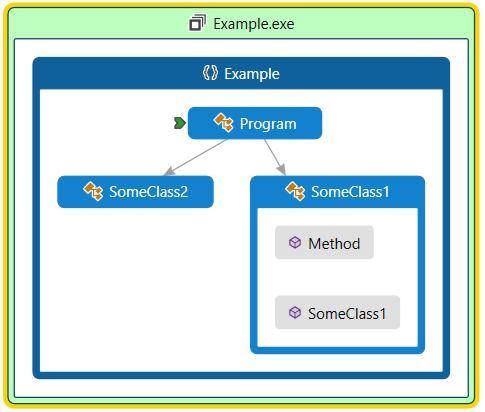
\includegraphics{CodeMap.PNG}
\caption{Графическое представление кода в CodeMap}
\end{figure}


\paragraph {Python Tutor}
Данный веб продукт имеет возможность анализировать учебные программы, состоящие из одного файла, на языках Python, Java, JavaScript и наглядно изображать их выполнение. Предназначен для визуализации выполнения программ, написанных в собственной онлайн среде разработки.  \\
С точки зрения визуализации данный инструмент позволяет.

\begin{itemize}

        \item { Отобразить пошаговое исполнение каждого метода, путем визуализации пошаговой работы интерпретатора. }
        
 \end{itemize}
Недостатком данного инструмента являются:

\begin{itemize}

        \item { Невозможность интеграции в среду разработки. }
        \item { Обязательное подключение к интернету. }
        \item { Невозможность других режимов синтаксического разбора, отличных от пошагового. }
        
 \end{itemize}

Ниже представлен результат работы данного инструмента (рис. 2).
\begin{figure}[h]
\label{Python}
\centering
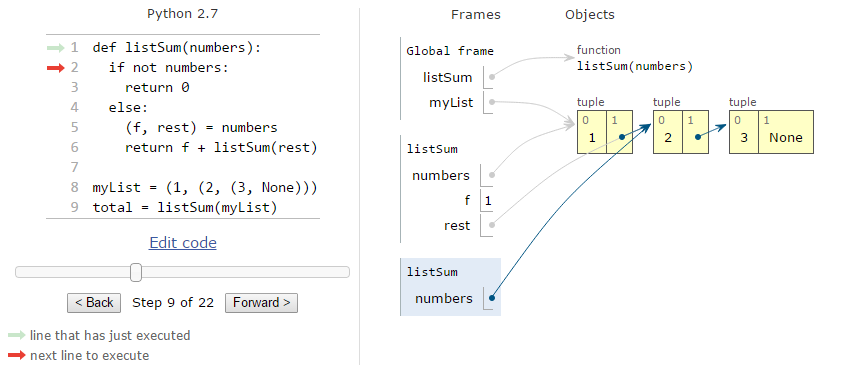
\includegraphics{PythonTutor.PNG}
\caption{Пример работы PythonTutor}
\end{figure}


\paragraph {Code Visual Editor}
Code Visual Editor - программа, способная анализировать исходный код и отображать его в виде блок-схемы. Программа анализирует языки программирования C, C++, Pascal, Perl, PHP, PL/SQL, POSIX shell, Power Script, T-SQL, Visual Basic/VBA, VB.NET, VBScript, and Qbasic/Basic.   \\
Достоинством продукта является.

\begin{itemize}

        \item { Возможность анализировать выделенную часть кода. }
        
 \end{itemize}
Недостатком данной программы являются.

\begin{itemize}

        \item { Отсутствие интеграции в среду разработки. }
        \item { Закрытый исходный код. }
        \item { Для каждого запуска требуется указывать параметры работы систем; }
        \item { Отсутствие возможности анализировать строковые выражения. }
        
 \end{itemize}

Ниже представлен результат работы данного инструмента (рис. 3).
\begin{figure}[h]
\label{CodeVisual}
\centering
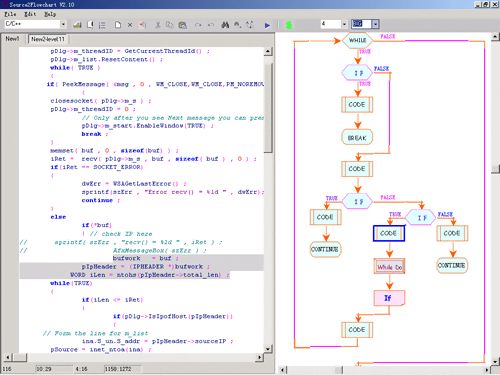
\includegraphics{CodeVisualEditor.png}
\caption{Пример работы Code Visual Editor}
\end{figure}


\paragraph {Code to FlowChart}
Code to FlowChart - продукт, генерирующий код в блок схему. Это помогает пользователям понять сложную структуру программы с помощью визуальных диаграмм. Code to FlowChart поддерживает языки программирования C, C++, VC++ and Pascal/Delphi.   \\
Достоинством продукта является.

\begin{itemize}

        \item { Подсветка выделенного кода в построенной блок-схеме. }
        \item { Цветовое выделение различных языковых конструкций. }
        
 \end{itemize}
Недостатком данной программы являются.
\newpage{}
\begin{itemize}

        \item { Отсутствие интеграции со средой разработки. }
        \item { Закрытый исходный код. }
        \item { Отсутствие возможности анализировать строковые выражения. }
        
 \end{itemize}

Ниже представлен результат работы данного инструмента (рис. 4).
\begin{figure}[h]
\label{CodeVisual}
\centering
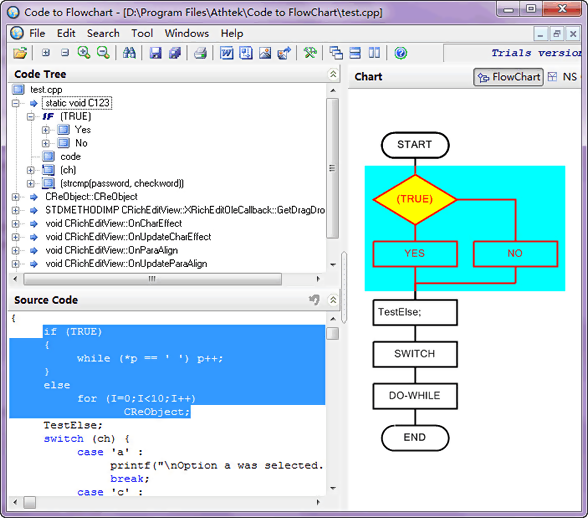
\includegraphics[width=\textwidth]{CodeToFlowChart.png}
\caption{Пример работы CodeToFlowChart}
\end{figure}


\newpage{}
\section{Постановка задачи}
    Целью данной работы является разработка компоненты, предназначенной для графического представления данных в среде разработки  Microsoft Visual Studio с последующей интеграцией в проект YaccConstructor. Данный модуль позволяет визуализировать структуру динамически формируемого выражения, что позволяет упростить поиск ошибок и поддержку кода. 
Для достижения поставленной цели были сформулированы следующие задачи.

\begin{itemize}

         \item { Изучить библиотеку для визуализации графов GraphX~\cite{wiki:GraphX}.}
        \item { Изучить плагин для Visual Studio, проводящий статический анализ кода Resharper. }
       \item { Создать графическую компоненту, встроенную в среду разработки Microsoft Visual Studio. }
        \item {Добавить компоненту в YC.ReSharper.AbstractAnalysis plugin~\cite{wiki:Plugin} с возможностью отрисовки графов в среде Microsoft Visual Studio.}
        \item{ Добавить в YC.ReSharper.AbstractAnalysis plugin возможность запускать визуализатор непосредственно в среде разработки Microsoft Visual Studio. }
        \item{ Добавить в YC.ReSharper.AbstractAnalysis plugin возможность просмотра требуемой информации в графическом виде, путем вывода графа. }
        \item { Ввиду того, что в коде может формироваться несколько строковых выражений, следует добавить в YC.ReSharper.AbstractAnalysis plugin возможность переключаться между графами различных формируемых выражений. }
 \end{itemize}
Ниже приведен пример кода и ожидаемого графа:\\
1 private void Go(int a, int b, int c)\\
2 \{\\
3 \ \ \ \ String s = "select ";\\
4 \ \ \ \ if (a > b) \{\\
5 \ \ \ \ \ \ \ \ s += "x from y";\\
6 \ \ \ \ \}\\
7 \ \ \ \ else \{\\
8 \ \ \ \ \ \ \ \ if (c > b) \{\\
9 \ \ \ \ \ \ \ \ \ \ \ \ s += "y from x";\\
10 \ \ \ \ \ \ \ \ \}\\
11 \ \ \ \ \ \ \ \ else \{\\
12 \ \ \ \ \ \ \ \ \ \ \ \ s += "y from z";\\
13 \ \ \ \ \ \ \ \ \}\\
14 \ \ \ \ \}\\
15 \ \ \ \ Program.ExecuteImmediate(s);\\
16 \}

\begin{figure}[h]
\label{CodeVisual}
\centering
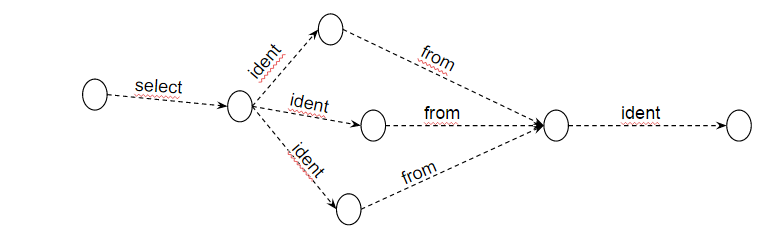
\includegraphics[width=\textwidth]{NeedGraph.PNG}
\caption{Ожидаемый граф}
\end{figure}

\newpage
\section{Основная часть}

В данном разделе будут рассмотрены подходы, примененные в разработке, и решения принятые в ходе работ.

На данном этапе компоненту можно разбить на три основные части, а именно:


\begin{itemize}

         \item { Подсистема создания диалогового окна. Данная подсистема отвечает за создание диалогового окна, встроенного в среду разработки Microsoft Visual Studio и логику взаимодействия с ним. Она основана на библиотеке ReSharper.SDK. Эта библиотека позволяет создавать собственные плагины для среды разработки Microsoft Visual Studio с сохранением дизайна данной среды разработки. }
        \item { Подсистема внутреннего представления графов. Пакет предназначен для удобного хранения всех составляющих компонент графов внутри плагина. Подсистема основана на библиотеках GraphX.Net и QuickGraph, имеющих соответственные классы для описания вершин, ребер и логической компоненты графов. }
       \item { Подсистема вывода графов в диалоговое окно. В её ответственность входит преобразование внутреннего представления графа в графическое с выводом в диалоговое окно. Данная подсистема основана на библиотеке GraphX.Net. Библиотека содержит набор алгоритмов визуализации графов, позволяет гибко конфигурировать устройство и внешний вид графа.
}
\end{itemize}
 
Для упрощения понимания взаимодействия компонент ниже изображена архитектура компоненты:
\newpage
\begin{figure}[t]
\label{Pack}
\centering
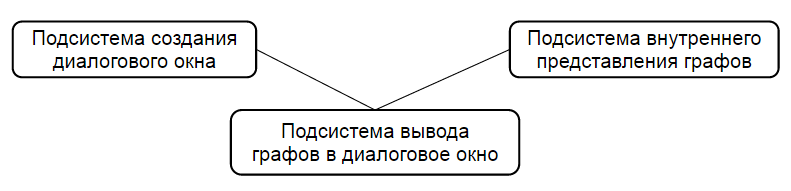
\includegraphics[width=\textwidth]{Packages.png}
\caption{Общая архитектура компоненты}
\end{figure}

В процессе создания компоненты была обнаружена проблема хранения графов. Изначально планировалось хранить графы внутри диалогового окна, но было обнаружено, что данная подсистема начинает работу после открытия окна, однако граф может быть сгенерирован до этого, в результате часть графов может быть утеряна. Было решено завести отдельное хранилище для графов, чтобы компонента, независимо от времени запуска уже могла предоставить разобранные выражения  в  виде визуализированных графов и никакие из них не были потеряны. Для отображения нескольких графов в главном окне компоненты был использован класс TabControl, который содержит в себе класс Tab из библиотеки System.Windows.Forms.Control. Такая организация позволяет переключаться между графами, а при появлении нового добавить его. Класс Tab хранит внутри себя граф и выводит его графическое представление. Также граф реагирует на действия пользователя над графом, а именно при наведении указателя типа “мышь” на одно из ребер оно выделяется цветом. 

Ввиду того, что конечного пользователя интересует не только граф выражения, но и возможность наблюдать в графе этапы генерации строкового выражения, для работы с графом из библиотеки GraphX.Net были использованы и доработаны классы Edge, Vertex, LogicCore, GraphArea, Graph для хранения любой текстовой информации о выражении на ребрах и вершинах графа и возможности визуализировать его. Для представления графов в проекте YaccConstructor используется класс из библиотеки QuickGraph, а GraphX.Net использует другой класс библиотеки QuickGraph, поэтому для представления графов был реализован конвертер графов. 

Главное окно компоненты реализовано с помощью библиотеки Rasharper.SDK. Эта библиотека позволяет создать	 элемент, полностью интегрированный в среду разработки Microsoft Visual Studio. Для реализации главного окна были использованы классы Descriptor, Registrar и реализован интерфейс IActionHandler. Класс Descriptor служит для описания нового объекта среды разработки. Реализация интерфейса отвечает за создание событий, когда пользователей вызывает компоненту, а класс WindowRegistrar обрабатывает эти события.

Для более удобного представления системы ниже представлена диаграмма классов:


\begin{figure}[h]
\label{Diagram}
\centering
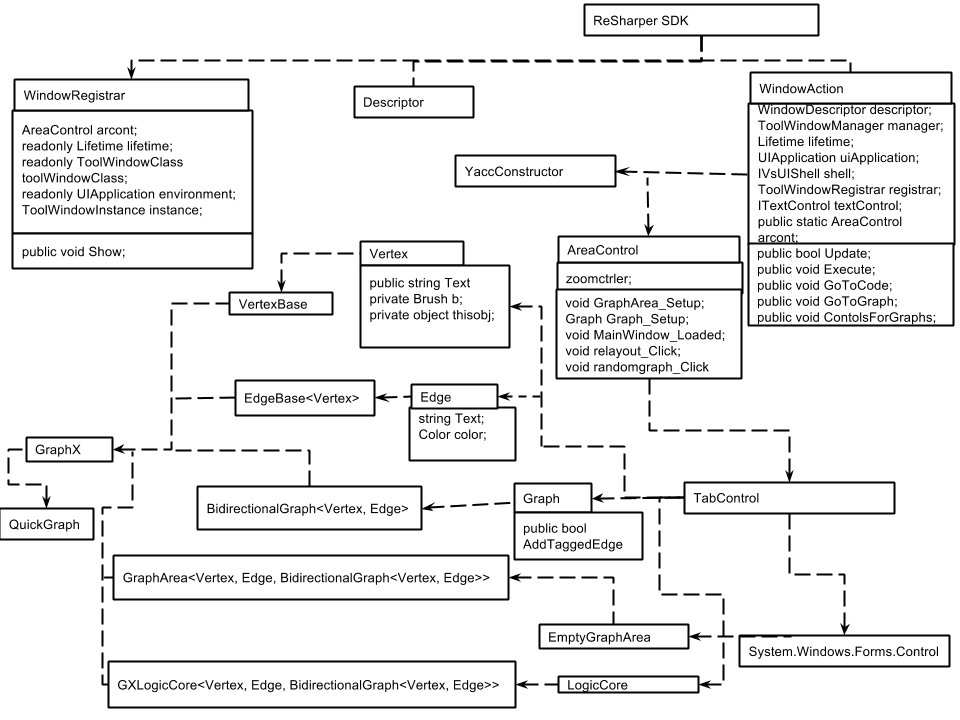
\includegraphics[width=\textwidth]{ClassDiagram.png}
\caption{Диаграмма классов}
\end{figure}

\newpage{}
По окончанию работы была проведена апробация плагина. Пример исходного кода и результаты можно увидеть ниже:\\
1 private void Go(int a, int b, int c)\\
2 \{\\
3 \ \ \ \ Program.ExecuteImmediate("select x from select x from select x from select\\
4 \ \ \ \ \ \ \ \ \ \ \ \ \ \ \ \ \ \ \ \ x from select x from select x from y");\\
5 \ \ \ \ Program.Eval("2 * (3 + 5)");\\
6 \ \ \ \ String s = "select ";\\
7 \ \ \ \ if (a > b) \{\\
8 \ \ \ \ \ \ \ \ s += "x from y";\\
9 \ \ \ \ \}\\
10 \ \ \ \ else \{\\
11 \ \ \ \ \ \ \ \ if (c > b) \{\\
12 \ \ \ \ \ \ \ \ \ \ \ \ s += "y from x";\\
13 \ \ \ \ \ \ \ \ \}\\
14 \ \ \ \ \ \ \ \ else \{\\
15 \ \ \ \ \ \ \ \ \ \ \ \ s += "y from z";\\
16 \ \ \ \ \ \ \ \ \}\\
17 \ \ \ \ \}\\
18 \ \ \ \ Program.ExecuteImmediate(s);\\
19 \ \ \ \ String stmt = "drop procedure";\\
20 \ \ \ \ if (c == 1) \{\\
21 \ \ \ \ \ \ \ \ Program.ExecuteImmediate(stmt + "prc2");\\
22 \ \ \ \ \}\\
23 \ \ \ \ else \{\\
24 \ \ \ \ \ \ \ \ Program.ExecuteImmediate(stmt + "prc1");\\
25 \ \ \ \ \}\\
26 \}\\

\begin{figure}[h]
\label{Hard}
\centering
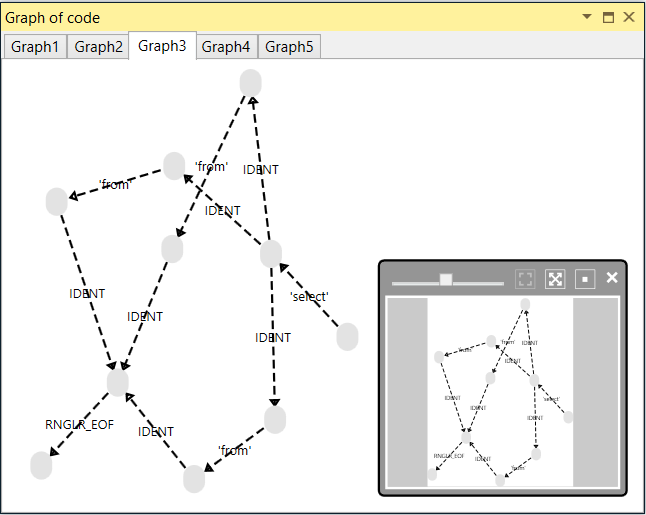
\includegraphics[width=\textwidth]{StrongGraph.PNG}
\caption{Полученный граф}
\end{figure}

\newpage{}
\section*{Заключение}
\subsection*{Результаты}
В результате работы была доработана библиотека GraphX для хранения требуемой информации на ребрах и вершинах графа, перехвата действий пользователя над графом. Была доработана компонента для передачи графа из анализатора в визуализатор. Доработан YC.ReSharper.AbstractAnalysis plugin для хранения требуемых графов, полученных в результате исполнения нескольких строковых выражений независимо от запуска визуализатора. Получившаяся система в результате работы позволяет следующее:

\begin{itemize}

         \item { Запуск визуализатора непосредственно в среде разработки Microsoft Visual Studio.}
        \item { Визуализация графов, полученных в результате работы алгоритмов  лексического и синтаксического анализа динамически формируемых выражений.
}
       \item { Возможность переключения между графами разных формируемых выражений. }
       \item {Возможность выделить рассматриваемое ребро графа.}
       \item {Возможность масштабирования графов.}
\end{itemize}

Исходный код проекта YaccConstructor можно найти на сайте\\
\href{https://github.com/YaccConstructor/YaccConstructor}https://github.com/YaccConstructor/YaccConstructor

Автор принимал участие под учетной записью m13oas.

\subsection*{Дальнейшее развитие}
Дальнейшим развитием компоненты является поддержка динамического изменения в окне количества графов. Также развитие взаимодействия с пользователем, а именно возможность навигации из графа в код и обратно из кода в граф. Не менее важно улучшение графического представления, путем добавления выделения цветом ошибочных путей, улучшение алгоритмов автоматической раскладки и выбор алгоритма раскладки графа непосредственно в компоненте. Добавление возможности сохранения графа в файл.

\bibliographystyle{ugost2008ls}
\bibliography{diploma.bib}
\end{document}
